\section{Trace Study}
\label{sec:trace}

Traces are used to collect information about the system workloads.
Traces can be collected at different layers in storage stack. Block
traces contain information about disk offset, number of blocks
accessed, Read/Write information and timestamp for every accessed I/O.
This information can be used to characterize the workloads and
identify I/O access patterns.  Trace analysis plays a crucial role in
identifying hot data blocks across different disks.The idea is to move
hot blocks to primary disk and serve most of the requests from most
energy efficient disk. Hence other disks can be spun/powered down for
long periods of time to achieve good power savings and increased
performance. A simple approach like counting the number of times a
particular block is accessed can be used to find the hotness of disk
blocks. Apart from this, I/O block traces can be used for variety of
other purposes.  For example, block trace analysis can be used to
tweak the design parameters like extent size and migration threshold.

Workloads which exhibit good data locality properties are most
suitable for this project. Workloads such as video server and file
server are likely to exhibit this property. The distribution of
popular files on disks may change dynamically but at any particular
instant, only a fraction of files the disk are popular in the case of
above workloads. A workload which is completely random I/O access
patterns could not benefit this approach as it could result in
frequent data migration between primary disks and secondary disks.
 
Currently, we use I/O traces for analysis and tweaking parameters. I/O
traces can also be used in offline mode to predict the hot blocks.
This approach is another option and we may implement this if time
permits. Also, to verify the correctness and working of our concept,
we replay the traces with and without green Multi-disk target and
compare the power consumption and I/O performance. 

\begin{figure}[ht]
\begin{centering}
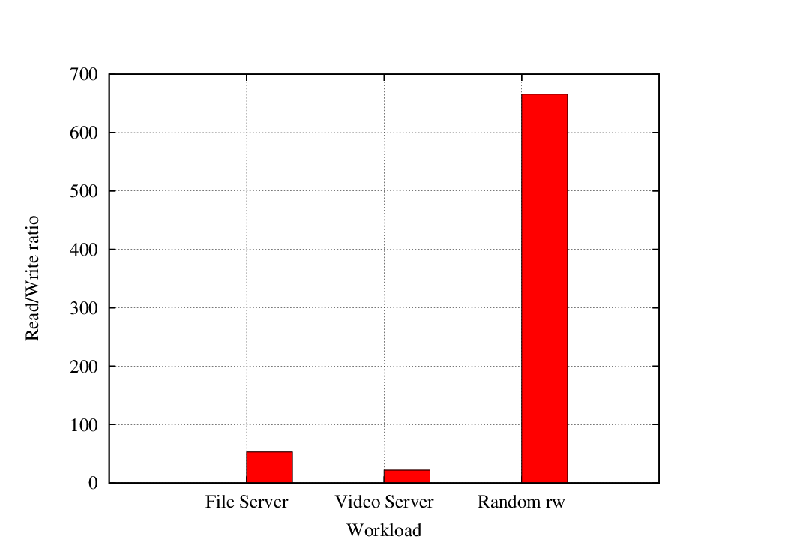
\epsfig{file=figures/rw.eps,width=1.00\linewidth}
\caption{Read/write ratio of video server, file server and random
  workloads.}
\label{fig:rwratio}
\end{centering}
\end{figure}

\begin{figure}[ht]
\begin{centering}
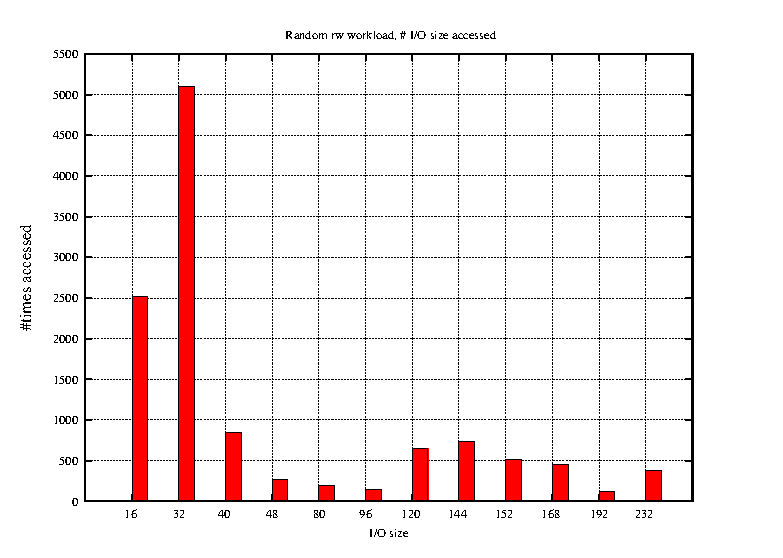
\epsfig{file=figures/randomrw_io_freq.eps,width=1.00\linewidth}
\caption{I/O size of the random workload.}
\label{fig:randomiosize}
\end{centering}
\end{figure}

I/O block traces have been collected for variety of workloads like
video server, file server and random workloads. The workloads were run
for a relatively long periods (for a few hours). Below, we present the
results for some preliminary analysis on the traces. Figure
\ref{fig:rwratio} shows Read/Write ratios for the above three
workloads.  We have collected the number of times a particular I/O
size was issued for the above three workloads. Figure
\ref{fig:randomiosize}, which shows the I/O size of the random
workloads, is one of them. All these workloads were generated using
Filebench and each workload runs for 2 hours. We used three different
physical disks with different power consumption and performance
characteristics to run these workloads. 

%%%%%%%%%%%%%%%%%%%%%%%%%%%%%%%%%%%%%%%%%%%%%%%%%%%%%%%%%%%%%%%%%%%%%%%%%%%%%%
%% For Emacs:
% Local variables:
% fill-column: 70
% End:
%%%%%%%%%%%%%%%%%%%%%%%%%%%%%%%%%%%%%%%%%%%%%%%%%%%%%%%%%%%%%%%%%%%%%%%%%%%%%%
%% For Vim:
% vim:textwidth=70
%%%%%%%%%%%%%%%%%%%%%%%%%%%%%%%%%%%%%%%%%%%%%%%%%%%%%%%%%%%%%%%%%%%%%%%%%%%%%%
% LocalWords:  SMR HDDs drive's SMRs
